\documentclass[border=4pt]{standalone}
\usepackage[T1]{fontenc}
\usepackage{lmodern}
\usepackage{amsmath}
\usepackage{pgfplots}
\pgfplotsset{compat=1.18}
\usepgfplotslibrary{groupplots,fillbetween}
\usetikzlibrary{calc,arrows.meta}
% one colour per kind of method, the same in every figure (Okabe-Ito)
\definecolor{neur}{HTML}{D55E00}   % neurons chosen by attribution
\definecolor{dirc}{HTML}{009E73}   % directions from the weird-vs-normal contrast
\definecolor{read}{HTML}{0072B2}   % readout methods and interventions chosen from readouts
\definecolor{pers}{HTML}{CC79A7}   % Assistant Axis / persona
\definecolor{ctrl}{HTML}{8C8C8C}   % random controls
\definecolor{meas}{HTML}{E69F00}   % measured outcome
\definecolor{ink}{HTML}{222222}
\pgfplotsset{
  every axis/.append style={clip=false, font=\small, axis line style={black!55}, tick style={black!55}, tick align=outside,
    label style={font=\small}, tick label style={font=\footnotesize}, title style={font=\small, align=center}},
  grid style={black!9, line width=0.4pt},
  every axis legend/.append style={font=\footnotesize, draw=none, fill=none},
  ci/.style={/pgfplots/error bars/x dir=both, /pgfplots/error bars/x explicit, /pgfplots/error bars/error bar style={line width=0.8pt}, /pgfplots/error bars/error mark=none},
  yci/.style={/pgfplots/error bars/y dir=both, /pgfplots/error bars/y explicit, /pgfplots/error bars/error bar style={line width=0.8pt}, /pgfplots/error bars/error mark=none},
}

\begin{document}
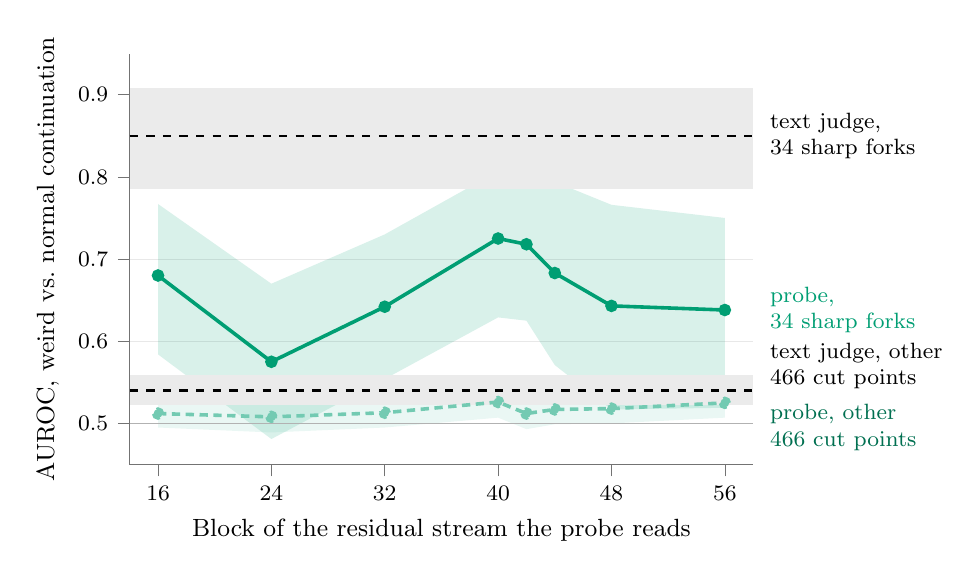
\begin{tikzpicture}
\begin{axis}[width=9.5cm, height=6.8cm, xmin=14, xmax=58, xtick={16,24,32,40,48,56}, ymin=0.45, ymax=0.95, ytick={0.5,0.6,0.7,0.8,0.9}, yticklabel style={/pgf/number format/.cd, fixed, precision=1}, axis x line*=bottom, axis y line*=left, ymajorgrids, xlabel={Block of the residual stream the probe reads}, ylabel={AUROC, weird vs.\ normal continuation}]
\draw[black!30, line width=0.5pt] (axis cs:14,0.5) -- (axis cs:58,0.5);
\fill[black!8] (axis cs:14,0.785) rectangle (axis cs:58,0.908);
\draw[black, dashed, line width=0.9pt] (axis cs:14,0.850) -- (axis cs:58,0.850);
\fill[black!8] (axis cs:14,0.522) rectangle (axis cs:58,0.559);
\draw[black, dashed, line width=0.9pt] (axis cs:14,0.540) -- (axis cs:58,0.540);
\addplot[name path=usharp, draw=none] coordinates {(16,0.767) (24,0.670) (32,0.730) (40,0.807) (42,0.809) (44,0.794) (48,0.766) (56,0.750)};\addplot[name path=dsharp, draw=none] coordinates {(16,0.584) (24,0.481) (32,0.554) (40,0.629) (42,0.625) (44,0.571) (48,0.517) (56,0.519)};\addplot[dirc, fill opacity=0.15] fill between[of=usharp and dsharp];\addplot[dirc, line width=1.3pt, mark=*, mark size=1.6pt] coordinates {(16,0.680) (24,0.575) (32,0.642) (40,0.725) (42,0.718) (44,0.683) (48,0.643) (56,0.638)};
\addplot[name path=uother, draw=none] coordinates {(16,0.530) (24,0.525) (32,0.532) (40,0.545) (42,0.530) (44,0.534) (48,0.537) (56,0.542)};\addplot[name path=dother, draw=none] coordinates {(16,0.495) (24,0.489) (32,0.495) (40,0.507) (42,0.493) (44,0.499) (48,0.500) (56,0.507)};\addplot[dirc!55, fill opacity=0.15] fill between[of=uother and dother];\addplot[dirc!55, line width=1.3pt, mark=*, mark size=1.6pt, densely dashed] coordinates {(16,0.512) (24,0.508) (32,0.513) (40,0.526) (42,0.512) (44,0.517) (48,0.518) (56,0.525)};
\node[font=\footnotesize, anchor=west, align=left] at (axis cs:58.5,0.850) {text judge,\\34 sharp forks};
\node[font=\footnotesize, anchor=west, align=left, dirc] at (axis cs:58.5,0.638) {probe,\\34 sharp forks};
\node[font=\footnotesize, anchor=west, align=left] at (axis cs:58.5,0.570) {text judge, other\\466 cut points};
\node[font=\footnotesize, anchor=west, align=left, dirc!70!black] at (axis cs:58.5,0.495) {probe, other\\466 cut points};
\end{axis}
\end{tikzpicture}
\end{document}
